%%%%%%%%%%%%%%%%%%%%%%%%%%%%%%%%%%%%%%%%%%%%%%%%%%%%%%%%%%%%%%%%%%%%%%
% How to use writeLaTeX:
%
% You edit the source code here on the left, and the preview on the
% right shows you the result within a few seconds.
%
% Bookmark this page and share the URL with your co-authors. They can
% edit at the same time!
%
% You can upload figures, bibliographies, custom classes and
% styles using the files menu.
%
%%%%%%%%%%%%%%%%%%%%%%%%%%%%%%%%%%%%%%%%%%%%%%%%%%%%%%%%%%%%%%%%%%%%%%

\documentclass[12pt]{article}

\usepackage{sbc-template}

\usepackage{graphicx,url}

%\usepackage[brazil]{babel}
\usepackage[utf8]{inputenc}


\sloppy

\title{Constructing a weak supervised dataset of Fine-Grained Emotions in Portuguese}

\author{Diogo Cortiz\inst{1,2}, Jefferson O. Silva\inst{2}, Flávio Rech
  Wagner\inst{2}, Jomi F. Hübner\inst{3} }


\address{Web Technology Study Center (Ceweb.br) - Brazilian Network Information Center (NIC.br) \\
  São Paulo - SP - Brazil
\nextinstitute
  Pontificia Universidade Católica de São Paulo (PUC-SP)\\
  São Paulo, SP, Brazil.
\nextinstitute
  Departamento de Sistemas e Computação\\
  Universidade Regional de Blumenal (FURB) -- Blumenau, SC -- Brazil
  \email{\{dcortiz\}@pucsp.br, R.Bordini@durham.ac.uk,
  jomi@inf.furb.br}
}

\begin{document}

\maketitle

\begin{abstract}
  This meta-paper describes the style to be used in articles and short papers
  for SBC conferences. For papers in English, you should add just an abstract
  while for the papers in Portuguese, we also ask for an abstract in
  Portuguese (``resumo''). In both cases, abstracts should not have more than
  10 lines and must be in the first page of the paper.
\end{abstract}

\begin{resumo}
  Este meta-artigo descreve o estilo a ser usado na confecção de artigos e
  resumos de artigos para publicação nos anais das conferências organizadas
  pela SBC. É solicitada a escrita de resumo e abstract apenas para os artigos
  escritos em português. Artigos em inglês deverão apresentar apenas abstract.
  Nos dois casos, o autor deve tomar cuidado para que o resumo (e o abstract)
  não ultrapassem 10 linhas cada, sendo que ambos devem estar na primeira
  página do artigo.
\end{resumo}


\section{Introduction}

Affective computing is the study of how computers can recognize, interpret and simulate human effects. According to Rosalind Picard, one of the pionners in this field, it is important to develop the ability to recognize, understand, and express emotions in computers if we want to have an intelligent and natural interaction between human and machines \cite{Rosalind2000}. We can develop affective computing technologies using different types of input, such as facial expression, voice, physiological data and language. The scope of this research, however, is delimited in the area of Natural Language Processing (NLP).

A common task in NLP is Sentiment Analysis which typically classify a text in three different categories: positive, negative, and neutral \cite{Drus2019}. Emotion Recognition task, however, is a more detailed NLP task. Rather than classifying text only into valence categories (positive, negative or neutral), it classifies text into granular emotional categories.

The scope of this research is concentrated in the area of fine-grained Emotion Recognition. In other words, the focus of the work is to study the creation of a corpus in Portuguese language that has a greater granularity of emotional categories, instead of just the valence categories.

\section{Related Work} 

There is an ongoing debate about the nature of human emotions, with different perspectives and theories. On one side is the theory of basic emotions, whose greatest exponent is the psychologist Paul Ekman. According to him, there are basic and universal emotions in humans that have unique features: such as facial expressions, signs, physiology and antecedent events \cite{Ekman1992}. 

There are several works in the area of NLP that are based on the theory of basic emotions to classify texts into defined categories of emotions, ranging from 4 (four) to 8 (eight) the number of categories. One of the studies adopted the 6 (six) basic emotions proposed by Ekman (\textit{joy, fear, anger, sadness, surprise,} and \textit{disgust}) to train an Emotion Recognition model \cite{Batbaatar2019}. Another researched added \textit{trust} and \textit{anticipation} emotions to the basic emotions, working with 8 (eight) basic emotion categories \cite{Sosea2020}.

However, there are other theories that challenge the proposition of basic emotions. Lisa Feldman Barrett proposed The Theory of Constructed emotion. Supported by positions from cognitive science and evidence from neuroscience experiments, the researcher argues that basic and universal emotions do not exist and that all emotional experience is constructed based on interoception and categorization process \cite{Barrett2016}.

Between those two antagonistic theories (The Basic Emotion Theory and The Theory of Constructed Emotion) an alternative perspective emerges: The Semantic Space Theory \cite{Cowen2021}. It is a computational approach that uses naturalistic stimuli and open-ended statistical techniques to capture emotional variations in behavior. Results suggest that more than 25 emotional classes have distinct profiles of previous expressions and events. Authors argue that these emotions are high-dimensional, categorical, and often blended.

Based on the Semantic Space Theory, a research that had the participation of one of the authors of the theory, created a dataset for training NLP models for the Emotion Recognition task. This is GoEmotions, a dataset with more than 58,000 English Reddit comments labeled for 27 categories of emotions and Neutral. The authors fine-tuned a BERT language model and achieved an average F1-score of .46 \cite{Demszky2020}.

Despite the average f1-score below .50, some classes scored above .70. It is a complex dataset with many categories that often have fuzzy boundaries among them. It is important to argue about the need for creating a fine-grained dataset, with more emotional categories, so that research in the Affective Computing area is not limited to Sentiment Analysis or to the limited categories proposed by the basic theory.

Although the GoEmotion dataset was released according to open data standards \cite{Demszky2020}, the scope of the corpus is limited to the English, which makes it difficult to use in applications in other languages. One of the challenges that the Machine Learning faces is dealing with low-resources, when the data available is not enough to train the models. This phenomenon can happen in specific domains of applications, but also in specific geographic regions.

In the area of NLP there is a lack of datasets and corpus available in many languages. This is the case of Portuguese, which has a small amount of Sentiment Analysis datasets when compared to English \cite{Pereira2021}. It's worth noting that we searched for dataset of fine-grained emotion, but we didn't find any in Portuguese.

\section{Objectives, Research Questions and Hypothesis}

The objective of this research is to study the creation of a corpus of fine-grained emotions for low resources languages, specifically the Portuguese. Due to limited financial resources, a specific objective of this work is to study the use of the weak supervision strategy to construct our corpus. Weak supervision is a strategy when there is no human annotation of each datapoint does not occur, but the labels are attributed using noisy and limited sources or specific rules. Then we proposed the following Research Question to guide our work:

RQ1: Is the weak supervision strategy suitable for building an NLP corpus for the fine-grained Emotion Recognition task in a low resources environment?

RQ2: What is a proper weak supervision approach to construct a corpus for  fine-grained Emotion Recognition task in NLP? 

One of our hypothesis is that a lexical-based approach can be an adequate strategy to collect samples for each of the categories of our dataset, using the Lexical Item (LI) as a criterion for defining the label in an adequate way for Portuguese. A second hypothesis is that the use of SOTA Machine Learning techniques (specifically Transformers based language models), combined with the application of masking techniques in the LI presented in the weak supervised corpus, can avoid the model to overfit during the learning phase. 

To answer RQ1 and RQ2 and validate our hypotheses, we prepared an experiment to create a weak supervised corpus in Portuguese and measure its performance by training a classification model. In the following sections we will describe our experimental protocol, including how we collected and weakly annotated the data, our model architecture, metrics and results. 

\section{Experimental Protocol}

Our experiment is composed by the following pipeline: defining emotion categories based on semantic space theory for Portuguese; selecting the lexical items related to each emotion category based on its definition; collecting the data; manually annotating a test dataset to create a golden standard; defining the model architecture; training the model and evaluating it on golden standard. Each of them is described in details in this paper.

\subsection{Defining Emotion Categories}

The emotion categories for this research were defined from a review of the GoEmotion work \cite{Demszky2020}. The review process had two stages and had the participation of a group of 7 (seven) researchers with different backgrounds (psychology, neuroscience, sociology, communications, cognitive science and computer science). In the first stage, during a working meeting, the researchers discussed and reviewed each of the emotions in English and proposed a translation into Portuguese based on the  definitions of each emotion. The result of this first stage was a translated list of terms with consensus among the reviewers.

The second stage was reviewing the categories definition in Portuguese to check if they were all consistent with the language. The researchers suggested changing the emotional category \textit{cuidado}, translated from \textit{caring} to \textit{compaixão}, as it is a more comprehensive and blended category in the Portuguese language. The second proposal was the removal of the emotion \textit{Realization}, in the sense of perceiving something, as it is not a much prevalent emotional category in the Portuguese language. Finally, there was a consensus among researchers to add the categories \textit{saudade} and \textit{inveja} to the list. The final list of emotional categories and their definitions are presented in Table 1.

\begin{table}
  \caption{Students' count per country of residence at the time of first participation}
  \label{tab:sts_by_countries}
  \begin{tabularx}{\textwidth}{X}
    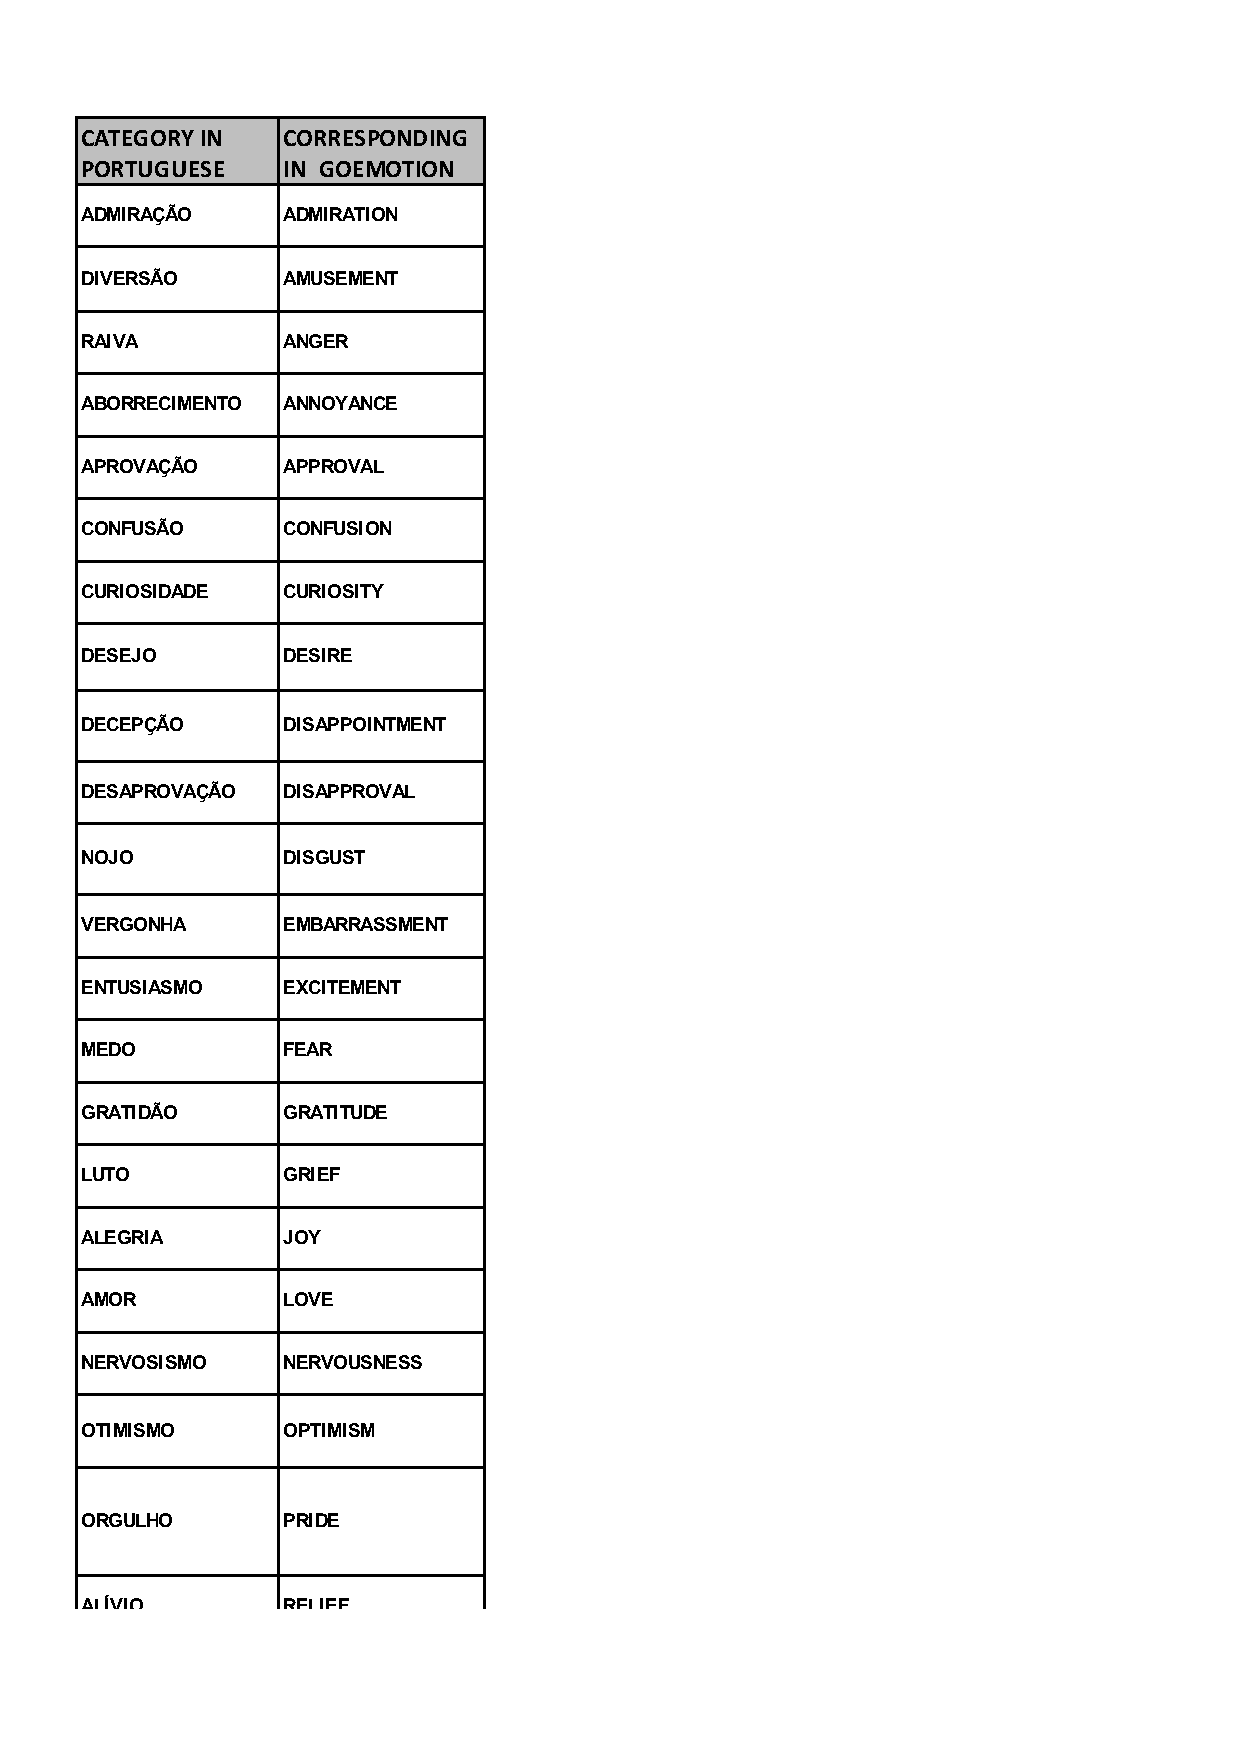
\includegraphics[trim=0cm 6.5cm 1cm 1.3cm, clip, width=\textwidth]{img-n-tables/EMOCOES}
  \end{tabularx}
\end{table}




- Explicar que herdamos as emoções do GoEmotion, mas adicionamos saudade,


\subsection{Selecting Lexical Items for weak supervision }
- Explicar o processo de Weaklabel (associação dos termos com as categorias de emoções - sinônimos e conjugações de verbos que tinham a ver com a definição de emoção utilizada)

\subsection{Collecting the data}

- A coleta foi feita no twitter entre os dias 23 e 24 de junho de 2016. 
- Descrever o processo de limpeza. Foram removidos hashtags, Links e replies.

- Descrever o tamanho da amostra total de treino e por emoções. 

\subsection{Golden standard for test dataset}

- Descrever que a amostra de test passou por um processo de anotação manual. Descrever o tamanho da amostra total e por emoções.



\subsection{Models}
- Descrever que o modelo utilizado foi a implementação BERT Bertimbau pré-treinado. 

- Foi feito o fine-tuning de três modelos

- O primeiro usou o dados de treinamento sem intervenção

- O segundo uso dados de treinamento no qual 30% dos datapoints foram mascarados. Ou seja, 30% dos termos utilizados para o WeakLabel foram trocados por [MASK]. Argumentar que a importância disso era evitar o overffiting por palavras específicas. 

- O terceiro modelo foi treinado mascarando todos os termos por [MASK]

\subsection{Parameters Settings}
Settings do modelo
- learning rate
- batchsize 
- epochs
- threshold 

\subsection{Metrics}
Descrever que a métrica de avaliação será a Precision, Recall and F1-score Macro (para o modelo e classes). 

\subsection{Results}
Apresentar o resultado dos três modelos treinados:

- Sem intervenção

- 30 por cento dos termos mascarados

- 100 por cento dos termos mascarados


\section{Conclusions}\label{sec:figs}


\begin{figure}[ht]
\centering
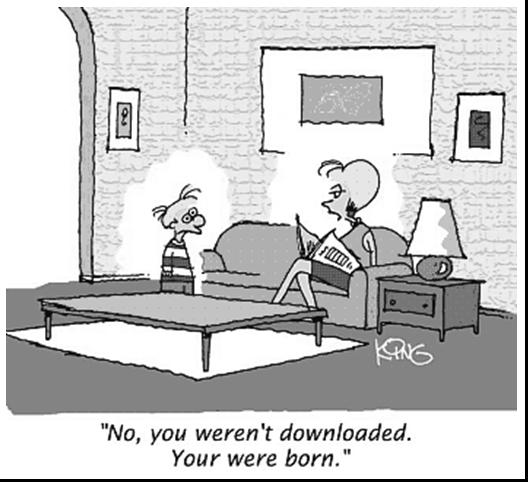
\includegraphics[width=.5\textwidth]{img/fig1.jpg}
\caption{A typical figure}
\label{fig:exampleFig1}
\end{figure}

\begin{figure}[ht]
\centering
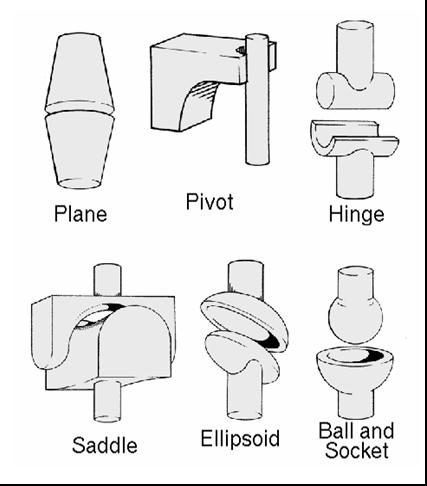
\includegraphics[width=.3\textwidth]{img/fig2.jpg}
\caption{This figure is an example of a figure caption taking more than one
  line and justified considering margins mentioned in Section~\ref{sec:figs}.}
\label{fig:exampleFig2}
\end{figure}

In tables, try to avoid the use of colored or shaded backgrounds, and avoid
thick, doubled, or unnecessary framing lines. When reporting empirical data,
do not use more decimal digits than warranted by their precision and
reproducibility. Table caption must be placed before the table (see Table 1)
and the font used must also be Helvetica, 10 point, boldface, with 6 points of
space before and after each caption.

\begin{table}[ht]
\centering
\caption{Variables to be considered on the evaluation of interaction
  techniques}
\label{tab:exTable1}
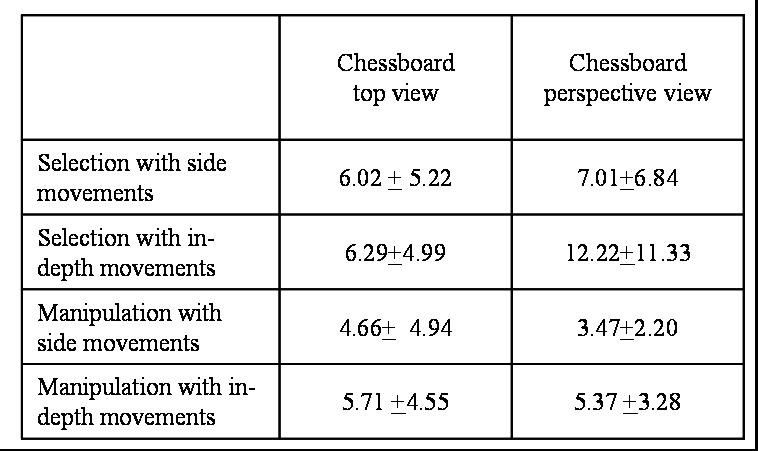
\includegraphics[width=.7\textwidth]{table.jpg}
\end{table}

\section{Images}

All images and illustrations should be in black-and-white, or gray tones,
excepting for the papers that will be electronically available (on CD-ROMs,
internet, etc.). The image resolution on paper should be about 600 dpi for
black-and-white images, and 150-300 dpi for grayscale images.  Do not include
images with excessive resolution, as they may take hours to print, without any
visible difference in the result.

\section{References}

Bibliographic references must be unambiguous and uniform.  We recommend giving
the author names references in brackets, e.g. \cite{knuth:84},
\cite{boulic:91}, and \cite{smith:99}.

The references must be listed using 12 point font size, with 6 points of space
before each reference. The first line of each reference should not be
indented, while the subsequent should be indented by 0.5 cm.

\bibliographystyle{sbc}
\bibliography{referencias}

\end{document}
